% User manual for the "New benchmarking model" tool.
% Paths are relative to this file; see manuals/_template/main.tex for the convention.
\input{../../shared/preamble.tex}
\graphicspath{ {../../../graphs/} }
\makeatletter
\def\input@path{ {../../../graphs/} }
\makeatother
% TikZ libraries used by the calculation-flow diagram in chapters/01_calculation.tex.
\usetikzlibrary{arrows.meta, positioning}
\begin{document}
	\title{Regumetrica \linebreak \emph{Beta version} \linebreak New benchmarking model user manual \linebreak Version 1.0 \\}
	\author{\href{https://www.regumetrica.com/um}{www.regumetrica.com/um}}
	\maketitle
\setcounter{page}{1}
\doublespacing

\tableofcontents
\newpage

\section*{Introduction}
\addcontentsline{toc}{section}{Introduction}
The New benchmarking model is a standalone tool for exploring Ei's proposed
benchmarking model for Swedish electricity distribution networks --- a model in
which efficiency is assessed on total expenditure (TOTEX) and the reference point
moves from the efficiency frontier to the third quartile of the sector. The tool
shows how a single company would be affected by the proposed model on its own,
holding everything else equal; it does not alter the current revenue-frame
calculation.

This manual will grow to cover the full tool. The present version documents the
calculation engine end to end.

%% Chapter: How the calculation works (capital base -> capital cost -> TOTEX ->
%% DEA -> efficiency requirement). Self-contained; \input from main.tex.
%% Audience: regulator staff and analysts/decision-makers at network companies,
%% not econometricians. Clarity first.

\section{How the calculation works}
\label{sec:calculation}

This chapter follows one company's data through the engine behind the New
benchmarking model, from its reported assets to a percentage on its revenue cap.
The calculation runs in four steps, shown in Figure~\ref{fig:flow}. Each step
feeds the next: the capital base becomes a capital cost; the capital cost joins
the operating costs to form \emph{TOTEX} (total expenditure); \emph{DEA} scores
TOTEX into an efficiency number between~0 and~1; and the tool turns that number
into an annual efficiency requirement.

\begin{figure}[H]
\centering
\resizebox{\textwidth}{!}{%
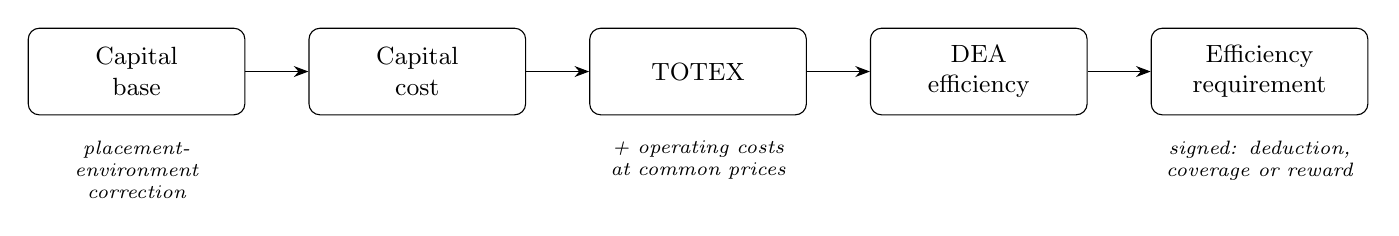
\begin{tikzpicture}[
    node distance=8mm,
    box/.style={draw, rounded corners, align=center, inner sep=5pt,
                minimum height=11mm, text width=24mm, font=\small},
    >={Stealth[scale=1.1]}]
  \node[box] (cb) {Capital\\ base};
  \node[box, right=of cb] (cc) {Capital\\ cost};
  \node[box, right=of cc] (tx) {TOTEX};
  \node[box, right=of tx] (ef) {DEA\\ efficiency};
  \node[box, right=of ef] (rq) {Efficiency\\ requirement};
  \draw[->] (cb) -- (cc);
  \draw[->] (cc) -- (tx);
  \draw[->] (tx) -- (ef);
  \draw[->] (ef) -- (rq);
  \node[font=\scriptsize\itshape, below=2mm of cb, text width=24mm, align=center]
        {placement-environment\\ correction};
  \node[font=\scriptsize\itshape, below=2mm of tx, text width=26mm, align=center]
        {+ operating costs\\ at common prices};
  \node[font=\scriptsize\itshape, below=2mm of rq, text width=26mm, align=center]
        {signed: deduction,\\ coverage or reward};
\end{tikzpicture}%
}
\caption{The four calculation steps. Each box is described in its own section below.}
\label{fig:flow}
\end{figure}

\begin{quote}
\small\itshape
A note on units. Every cost figure in this chapter is annual and expressed in
\emph{tkr} (thousands of SEK). Network losses are valued in SEK per MWh and
converted to tkr. Efficiency scores and requirements are dimensionless.
\end{quote}


%% ---------------------------------------------------------------------------
\subsection{Step 1 --- From the capital base to a capital cost}
\label{sec:step1}

A company's \emph{capital base} is the regulated value of its physical assets ---
cables, substations, meters, transformers, and so on. The current regulation
already converts this base into an annual \emph{capital cost} using the
established method (asset ages, depreciation, and the regulatory rate of return).
The new benchmarking model reuses that same conversion. It changes only one thing
beforehand: it levels out cost differences that come from \emph{where} an asset
is placed rather than from how efficiently the company is run.

\paragraph{Why a placement-environment correction.}
Two identical cables can have very different book values purely because of their
surroundings. A cable buried in a dense city centre is far more expensive per
kilometre than the same cable in open countryside, because the ground works,
permits, and reinstatement cost more --- not because the operator chose a costlier
cable. If the benchmarking model compared raw capital costs, a company serving a
city would look ``inefficient'' for reasons entirely outside its control. The
correction removes that distortion so that companies are compared on a level
footing.

\paragraph{What the correction does.}
The tool re-prices two asset types down to a common reference environment:

\begin{itemize}
  \item \textbf{Underground cable} (\emph{jordkabel}) is levelled to the
        \emph{rural-normal} (\emph{landsbygd normal}) cost level. City, town
        (\emph{tätort}), and difficult-terrain cables are brought down to what the
        same cable type would cost in rural-normal conditions.
  \item \textbf{Substations} (\emph{nätstation}) are levelled to the
        \emph{outside-town} level by removing the explicit city/town surcharge
        (\emph{City- och tätortstillägg}) that Ei's price list books separately.
\end{itemize}

The correction only ever lowers an expensive environment toward the reference; it
never raises a cheaper-than-reference asset. After the asset values are adjusted,
the tool re-runs the standard capital-cost conversion on the corrected base. The
result is an \emph{environment-adjusted capital cost} per company that enters
TOTEX in the next step.

\begin{quote}
\small
\textbf{Reading the result.} A company with a lot of urban cable or many town
substations will see its capital cost fall under this step --- that fall is the
size of the placement penalty being removed, not an efficiency gain.
\end{quote}


%% ---------------------------------------------------------------------------
\subsection{Step 2 --- Building TOTEX}
\label{sec:step2}

\emph{TOTEX} is the single, all-in annual cost the new model measures each company
by. Where the current efficiency benchmark looks mainly at controllable operating
cost, the proposed model puts \emph{all} relevant costs --- operating and capital
--- into one figure. The tool builds it as a sum of four pieces:

\begin{equation}
\boxed{\;
\begin{aligned}
\text{TOTEX} ={}&
  \underbrace{\text{controllable cost} + \text{losses at a common price}
  + \text{selected non-controllable cost}}_{\text{operating cost}} \\[2pt]
  &+\ \underbrace{\text{adjusted capital cost}}_{\text{from Step 1}}
\end{aligned}
\;}
\end{equation}

Each piece is explained below.

\begin{description}
  \item[Controllable cost.] The company's adjustable operating cost, taken
        unchanged from the current model's figure (the indexed 2018--2021
        average). Reusing it keeps the comparison ``apples to apples'': the new
        and current models share the exact same controllable number, so any
        difference in outcome comes from the model design, not from re-measuring
        costs.

  \item[Losses at a common price.] Every network loses some energy in
        transmission. The cost of replacing that energy depends heavily on the
        local electricity price, which varies by price area and is outside the
        operator's control. To avoid penalising companies in expensive price
        areas, the model values each company's physical losses at a single
        \emph{common price} rather than its actual purchase price:
        \begin{equation}
          \text{loss cost} \;=\; \text{loss share} \times \text{common price}
          \times \text{energy fed in},
        \end{equation}
        with the common price set to \SI{753.44}{kr/MWh} in the main model
        (adjustable in the Experiment panel).

  \item[Selected non-controllable cost.] A defined set of costs the operator
        cannot influence but that still belong in a total-cost comparison: grid
        subscription, grid connection, feed-in compensation, and capacity
        reserve. Regulatory fees are excluded entirely, and network-loss costs
        are excluded here because they are already captured at the common price
        above.

  \item[Adjusted capital cost.] The environment-adjusted capital cost from
        Step~1.
\end{description}

The first three pieces together are the model's \emph{operating} cost; adding the
capital cost gives TOTEX. This single number is the only cost input the
efficiency analysis sees.


%% ---------------------------------------------------------------------------
\subsection{Step 3 --- Scoring efficiency with DEA}
\label{sec:step3}

\emph{Data Envelopment Analysis} (DEA) is the technique that turns costs and
outputs into a single efficiency score. The intuition is simple: a company is
efficient if it delivers a lot of ``service'' for its cost, and inefficient if a
peer delivers as much service for less.

\paragraph{Inputs and outputs.}
In the new model each company is described by:
\begin{itemize}
  \item \textbf{one input} --- its TOTEX from Step~2 (the cost side); and
  \item \textbf{several outputs} --- measures of how much network service it
        provides: number of customers, peak power, number of substations,
        delivered energy at low and high voltage, and the physical length of its
        lines (\emph{ledningslängd}).
\end{itemize}
Line length is included so that companies covering large, sparse areas --- which
genuinely need more network per customer --- are not scored as wasteful for it.

\paragraph{How the score is formed.}
DEA compares every company against the best-performing combinations of its peers
and produces an \emph{efficiency score} between~0 and~1:

\begin{itemize}
  \item a score of \textbf{1} means the company sits on the efficiency
        \emph{frontier} --- no peer (or combination of peers) delivers its outputs
        for less cost;
  \item a score \textbf{below 1}, say~0.90, means peers achieve the same outputs
        for about 90\% of this company's cost --- a~10\% efficiency gap.
\end{itemize}

\paragraph{Outliers.}
A few companies have unusual data that would distort the comparison. The model
flags these as \emph{outliers} using a standard statistical rule and excludes them
from setting the benchmark in Step~4. They are still scored and still receive an
outcome --- they simply do not influence the threshold the others are measured
against.

No knowledge of the underlying mathematics is needed to read the results: the
score is best understood as ``the share of this company's cost that an efficient
peer would need to deliver the same service.''


%% ---------------------------------------------------------------------------
\subsection{Step 4 --- From efficiency to an annual requirement}
\label{sec:step4}

The final step converts each company's efficiency score into an annual
\emph{efficiency requirement}: a percentage applied to the revenue cap. This step
is where the proposed model differs most sharply from today's, so we first describe
the change in principle, then give the formula, and finally state clearly what is
confirmed by Ei and what is our own working interpretation.

\paragraph{The change in principle.}
\begin{itemize}
  \item \textbf{Today}, the reference point is the \emph{frontier} (a score
        of~1). Every company is measured by how far below the frontier it sits, so
        every company receives a deduction --- the only question is how large.
  \item \textbf{In the proposed model}, the reference point moves from the
        frontier to the \emph{third quartile} of the efficiency distribution,
        written $E_{75}$ --- the score at the 75th percentile. A company is now
        measured by its \emph{signed gap} to that benchmark, so the outcome can go
        either way:
        \begin{itemize}
          \item below $E_{75}$ \,$\Rightarrow$\, a \textbf{deduction} (the revenue
                cap is lowered);
          \item exactly at $E_{75}$ \,$\Rightarrow$\, \textbf{full cost coverage}
                (no change);
          \item above $E_{75}$ \,$\Rightarrow$\, a \textbf{reward} (the revenue
                cap is raised).
        \end{itemize}
\end{itemize}
Because the benchmark is the 75th percentile, the most efficient quarter of the
sector receives full coverage or a reward, and the threshold recalibrates each
period as the sector's efficiency distribution shifts.

\paragraph{The formula.}
Let $E_i$ be a company's efficiency score and $E_{75}$ the third-quartile
benchmark (computed over non-outliers). The signed gap is $E_{75}-E_i$. The annual
requirement is:

\begin{equation}
\boxed{\;
\text{annual requirement}
= \Bigl(1 + \operatorname{clip}\!\left(E_{75}-E_i,\ \pm c\right)\times s\Bigr)^{1/p} - 1
\;}
\end{equation}

with the main-model settings
\[
\underbrace{c = 0.30}_{\text{gap cap}}, \qquad
\underbrace{s = \tfrac{1}{2}\times\tfrac{4}{8} = 0.25}_{\substack{\text{customer sharing}\ \times\\ \text{period / realisation time}}}, \qquad
\underbrace{p = 4}_{\text{years in period}} .
\]

A \textbf{positive} requirement is a deduction; a \textbf{negative} one is a
reward. The gap is capped symmetrically at $\pm 0.30$, which holds the largest
possible deduction at \textbf{+1.82\,\%/yr} --- the same ceiling as today's model,
so the two stay numerically anchored. There is no floor: full coverage at the
benchmark replaces the small minimum deduction the current model applies.

\paragraph{What is confirmed versus interpreted.}
Ei has published the \emph{direction} of the reform but not its full
specification. Table~\ref{tab:confirmed} separates what the model implements on
firm ground from what rests on our reading of Ei's intent. The settings in the
``interpretation'' column are the ones most likely to change once Ei publishes the
final method, and they are the parameters exposed for sensitivity testing.

\begin{table}[H]
\centering
\footnotesize
\begin{threeparttable}
\caption{What the requirement step rests on}
\label{tab:confirmed}
\begin{tabular}{@{}p{7.3cm}p{7.3cm}@{}}
\toprule
\textbf{Confirmed by Ei} & \textbf{Our working interpretation} \\
\midrule
The reference moves from the frontier to the third quartile ($E_{75}$); the
threshold is relative and recalculated each period.
& The outcome is \emph{linear in the cardinal gap} $E_{75}-E_i$ (rather than
rank-based). \\[4pt]
The top quarter of companies receive full cost coverage or more.
& A customer-sharing factor of $0.50$ carries over from today's model. \\[4pt]
The realisation time stays at 8 years.
& The cap on the outcome is symmetric at $\pm 0.30$ (Ei lists the cap as an open
question). \\[4pt]
The outcome is two-sided --- it can be a deduction \emph{or} a reward.
& Rewards above $E_{75}$ are scaled by the same factor as deductions below it
(symmetry is not yet specified). \\
\bottomrule
\end{tabular}
\begin{tablenotes}
\item Ei refers to the British RIIO-ED2 model for the third-quartile choice. ED2
adds a separate ongoing efficiency requirement and a glide path toward the 85th
percentile; the Swedish proposal, as described so far, includes neither.
\end{tablenotes}
\end{threeparttable}
\end{table}


%% ---------------------------------------------------------------------------
\subsection{A worked example}
\label{sec:example}

To see the steps connect, follow one fictional company, ``Nät~AB,'' through the
whole chain. The figures are illustrative round numbers, not real data.

\paragraph{Steps 1--2: building TOTEX.}
Nät~AB serves a partly urban area, so the placement-environment correction in
Step~1 removes a city/town penalty, lowering its capital cost from
\SI{100000}{} to \SI{92000}{tkr}. Its operating pieces and the resulting TOTEX
are shown in Table~\ref{tab:example-totex}.

\begin{table}[H]
\centering
\footnotesize
\begin{threeparttable}
\caption{Nät~AB: building TOTEX (all figures annual, tkr)}
\label{tab:example-totex}
\begin{tabular}{@{}lr@{}}
\toprule
\textbf{Component} & \textbf{Value} \\
\midrule
Controllable cost (reused from current model)        & 60\,000 \\
Losses at the common price\tnote{a}                  & 15\,069 \\
Selected non-controllable cost                       & 13\,000 \\
\midrule
\textit{Operating cost (subtotal)}                   & \textit{88\,069} \\
Environment-adjusted capital cost (Step~1)           & 92\,000 \\
\midrule
\textbf{TOTEX (single DEA input)}                    & \textbf{180\,069} \\
\bottomrule
\end{tabular}
\begin{tablenotes}
\item[a] $0.04$ loss share $\times$ \SI{753.44}{kr/MWh} $\times$
\SI{500000}{MWh} fed in $=\SI{15069}{tkr}$.
\end{tablenotes}
\end{threeparttable}
\end{table}

\paragraph{Steps 3--4: score and outcome.}
DEA scores Nät~AB at $E_i = 0.92$. Suppose the sector's third-quartile benchmark
is $E_{75} = 0.95$. Nät~AB sits just below the benchmark, so it faces a small
deduction:
\[
E_{75}-E_i = 0.95 - 0.92 = +0.03
\quad\Rightarrow\quad
\bigl(1 + 0.03 \times 0.25\bigr)^{1/4} - 1 = +0.19\,\%\text{/yr (deduction).}
\]

The sign is what matters. Table~\ref{tab:example-outcomes} contrasts Nät~AB with
two hypothetical peers --- one above the benchmark and one far below it --- to show
the full range of the mechanic.

\begin{table}[H]
\centering
\footnotesize
\begin{threeparttable}
\caption{How the same benchmark produces different outcomes ($E_{75}=0.95$)}
\label{tab:example-outcomes}
\begin{tabular}{@{}lccl@{}}
\toprule
\textbf{Company} & \textbf{Score $E_i$} & \textbf{Annual outcome} & \textbf{Meaning} \\
\midrule
Peer above benchmark   & 0.98 & $-0.19\,\%$/yr & reward (cap raised) \\
\textbf{Nät~AB}        & 0.92 & $+0.19\,\%$/yr & deduction (cap lowered) \\
Peer far below         & $\le 0.65$ & $+1.82\,\%$/yr & deduction at the cap \\
\bottomrule
\end{tabular}
\begin{tablenotes}
\item A company exactly at $E_{75}=0.95$ would get $0\,\%$ --- full cost coverage.
The maximum deduction of $+1.82\,\%$/yr is reached once the gap hits the
$0.30$ cap (here, at a score of $0.65$ or below).
\end{tablenotes}
\end{threeparttable}
\end{table}

Reading the chain end to end: Nät~AB's assets become an environment-adjusted
capital cost; that cost joins its operating costs to form a TOTEX of
\SI{180069}{tkr}; DEA scores that TOTEX against the sector at $0.92$; and because
$0.92$ is just below the third-quartile benchmark of $0.95$, the proposed model
applies a modest \SI{0.19}{\percent} annual deduction to the revenue cap. Had
Nät~AB been more efficient than the benchmark, the same machinery would have
produced a reward instead.


\bibliographystyle{aer}
\bibliography{references}

\end{document}
